\documentclass[12pt,a4paper]{article}
\usepackage{graphicx}
\usepackage{wrapfig}

\title{Praktikum Physik - Erzwungene Schwingungen}
\author{Simon Marti, Patricia Schwab, Mirco Kocher}
\date{09.03.2012}

\parindent=0pt 
\begin{document}
\maketitle

%%
% Ziel
%%
\section*{Ziel}
Messung der Eigenfrequenz der freien Schwingung bei unterschiedlichen D\"ampfungen und Bestimmung der D\"ampfungskonstante.

%%
% Motivation
%%
\section*{Motivation}
Der Versuch der erwungenen Schwingungen verschafft einen guten \"Uberblick \"uber das Gebiet der Differentalgleichungen. Ausserdem k\"onnen die gemessenen Daten graphisch auf logarithmischem Papier dargestellt werden. 

%%
% Theorie
%%
\section*{Theorie}
Die Periodendauer $T$ ist durch folgende Formel gegeben
\begin{equation}
T = \frac{Sekunden}{Perioden} \mbox [{s}]
\end{equation}
Die D\"ampfungskonstante $\alpha$ l\"asst sich durch folgende Formel absch\"atzen
\begin{equation}
\alpha = \frac{\ln\left( \frac{\varphi(n_{max} \cdot T)}{\varphi(n_{min} \cdot T)}\right)}{-T\cdot (n_{max} - n_{min})} \mbox [{s}^{-1}]
\end{equation}
Die Winkelgeschwindigkeit $\omega_0$ l\"asst sich folgendermassen bestimmen
\begin{equation}
\omega_0 = \frac{2\pi}{T} \mbox[{rad \cdot s}^{-1}]
\end{equation}
Ged\"ampfte harmonische Schwingung
\begin{equation}\label{eq:phi}
\varphi(t) = Ae^{-\alpha t}cos(\omega t - \beta)
\end{equation}
Die Resonanzfrequenz $\omega_0$ ist gegeben durch
\begin{equation}\label{eq:omega}
\Omega_R = \sqrt{\omega_0^2 - 2\alpha^2} \mbox [{s}^{-1}]
\end{equation}
Die Resonanzkurve l\"asst sich durch folgende Formel beschreiben
\begin{equation}\label{eq:a}
A(\varepsilon) = \frac{M_0}{2J\omega_0\sqrt{\varepsilon^2 + \alpha^2}}
\end{equation}
wobei $\varepsilon = \Omega - \omega_0$, $J$ dem Tr\"agheitsmoment und $M_0$ dem Drehmoment entspricht.

%%
% Experiment 1
%%
\section*{Experiment I}

% Aufbau und Ablauf
\subsection*{Aufbau und Ablauf}
\begin{center}
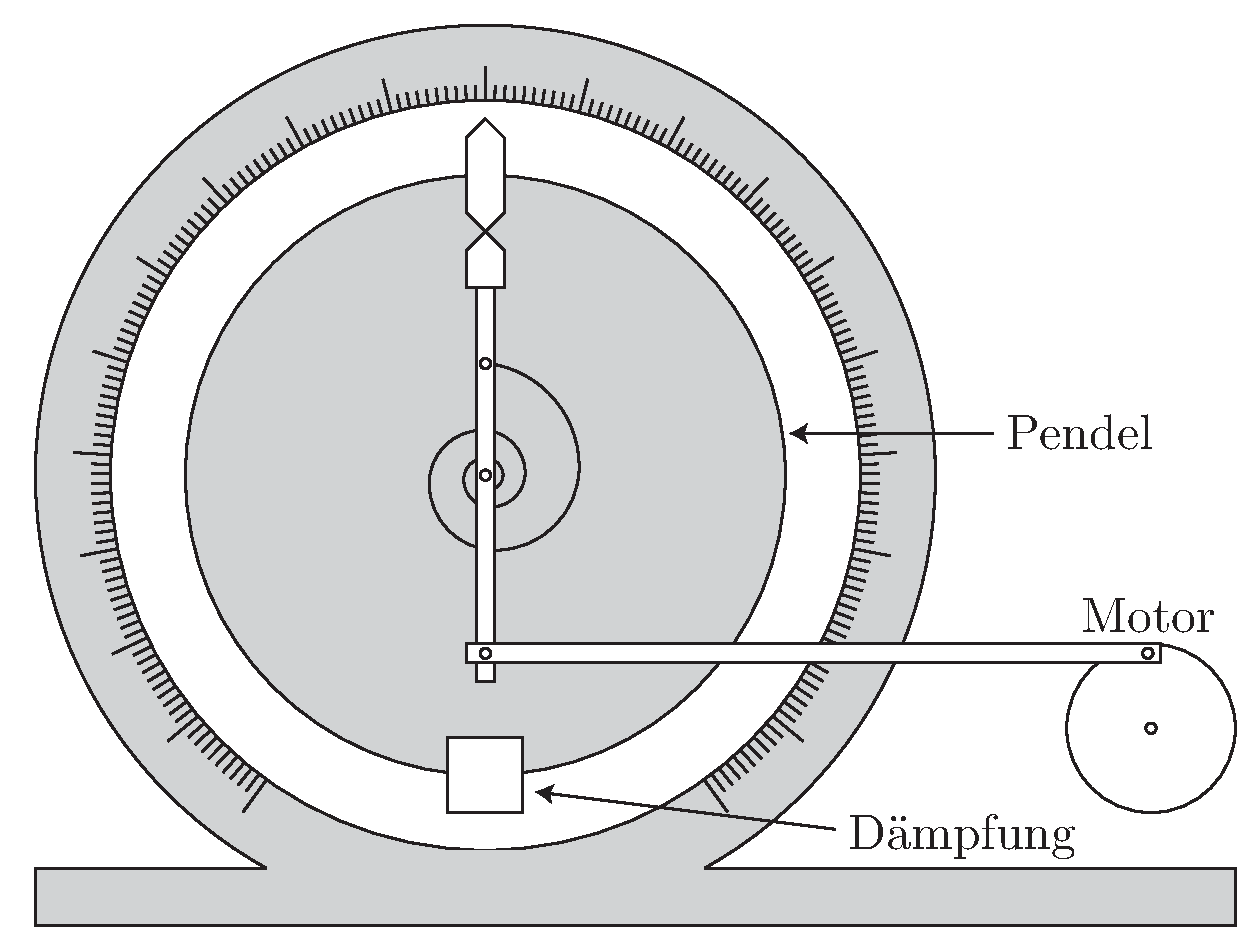
\includegraphics[width=13cm]{illustration.pdf}
\end{center}
Die Apparatur besteht aus einer vertikal stehenden Drehscheibe mit r\"ucktreibender Spiralfeder dessen Auslenkung an einer Skala abgelesen werden kann. Zwei Drahtspulen befinden sich beidseitig der Scheibe und wirken als Wirbelstrombremse deren St\"arke durch die Stromzufuhr geregelt werden kann. Ein Motor mit kontinuierlich verstellbarer Drehfrequenz liefert ein periodisches, externes Moment indem das feste Ende der Spiralfeder bewegt wird. Die Amplitude des Pendels wird jeweils von Patricia an der eingebauten Skala abgelesen, die Frequenz des Pendels und des Motors wird bestimmt indem Simon mir einer Stoppuhr zehn Perioden misst.

Beim ersten Experiment wird die Amplitude des Pendels in mehreren aufeinanderfolgenden Schwingungszyklen f\"ur verschiedene Dämpfungen gemessen. Das Pendel wurde jeweils bis zum Wert 9 auf der Skala ausgelenkt.

% Rohdaten
\subsection*{Rohdaten}
\subsubsection*{Ohne D\"ampfung}
Erste Messung

\vspace{3pt}
\begin{tabular}{|l|l|l|l|l|l|l|l|l|l|}
\hline
$A_{0}$&$A_{1}$&$A_{2}$&$A_{3}$&$A_{4}$&$A_{5}$&$A_{6}$&$A_{7}$&$A_{8}$&$A_{9}$\\
\hline
9.0&8.8&8.7&8.5&8.4&8.2&8.1&8.0&7.8&7.7\\
\hline
\hline
$A_{10}$&$A_{11}$&$A_{12}$&$A_{13}$&$A_{14}$&$A_{15}$&$A_{16}$&$A_{17}$&$A_{18}$&$A_{19}$\\
\hline
7.6&7.4&7.3&7.2&7.0&6.9&6.7&6.6&6.5&6.3\\
\hline
\hline
$A_{20}$&$A_{21}$&$A_{22}$&$A_{23}$&$A_{24}$&$A_{25}$&$A_{26}$&$A_{27}$&$A_{28}$&$A_{29}$\\
\hline
6.2&6.1&5.9&5.8&5.7&5.5&5.4&5.3&5.1&5.0\\
\hline
\end{tabular}

\vspace{10pt}
Zweite Messung

\vspace{3pt}
\begin{tabular}{|l|l|l|l|l|l|l|l|l|l|}
\hline
$A_{0}$&$A_{1}$&$A_{2}$&$A_{3}$&$A_{4}$&$A_{5}$&$A_{6}$&$A_{7}$&$A_{8}$&$A_{9}$\\
\hline
9.0&8.9&8.7&8.5&8.4&8.3&8.1&7.9&7.8&7.6\\
\hline
\hline
$A_{10}$&$A_{11}$&$A_{12}$&$A_{13}$&$A_{14}$&$A_{15}$&$A_{16}$&$A_{17}$&$A_{18}$&$A_{19}$\\
\hline
7.5&7.3&7.2&7.0&6.9&6.7&6.6&6.5&6.4&6.2\\
\hline
\hline
$A_{20}$&$A_{21}$&$A_{22}$&$A_{23}$&$A_{24}$&$A_{25}$&$A_{26}$&$A_{27}$&$A_{28}$&$A_{29}$\\
\hline
6.1&5.9&5.8&5.7&5.5&5.4&5.3&5.2&5.0&4.8\\
\hline
\end{tabular}

\vspace{10pt}
10$T$ = 20.0s

\subsubsection*{Mit D\"ampfung 0.45A}
Erste Messung

\vspace{3pt}
\begin{tabular}{|l|l|l|l|l|l|l|l|l|l|}
\hline
$A_{0}$&$A_{1}$&$A_{2}$&$A_{3}$&$A_{4}$&$A_{5}$&$A_{6}$&$A_{7}$&$A_{8}$&$A_{9}$\\
\hline
9.0&7.1&5.7&4.5&3.5&2.7&2.2&1.7&1.4&1.0\\
\hline
\end{tabular}

\newpage
Zweite Messung

\vspace{3pt}
\begin{tabular}{|l|l|l|l|l|l|l|l|l|l|}
\hline
$A_{0}$&$A_{1}$&$A_{2}$&$A_{3}$&$A_{4}$&$A_{5}$&$A_{6}$&$A_{7}$&$A_{8}$&$A_{9}$\\
\hline
9.0&7.2&5.8&4.5&3.5&2.7&2.1&1.6&1.2&0.9\\
\hline
\end{tabular}

\vspace{10pt}
10$T$ = 20.0s

\subsubsection*{Mit D\"ampfung 0.6A}
Erste Messung

\begin{tabular}{|l|l|l|l|l|l|l|l|l|l|}
\hline
$A_{0}$&$A_{1}$&$A_{2}$&$A_{3}$&$A_{4}$&$A_{5}$&$A_{6}$&$A_{7}$&$A_{8}$&$A_{9}$\\
\hline
9.0&6.0&4.0&2.6&1.7&1.1&0.6&0.4&0.2&0.1\\
\hline
\end{tabular}
\vspace{10pt}

Zweite Messung

\vspace{3pt}
\begin{tabular}{|l|l|l|l|l|l|l|l|l|l|}
\hline
$A_{0}$&$A_{1}$&$A_{2}$&$A_{3}$&$A_{4}$&$A_{5}$&$A_{6}$&$A_{7}$&$A_{8}$&$A_{9}$\\
\hline
9.0&6.0&4.0&2.7&1.8&1.2&0.7&0.4&0.3&0.1\\
\hline
\end{tabular}

\vspace{10pt}
10$T$ = 20.0s

% Auswertung
\subsection*{Auswertung}
Der logaritmische zeitliche Verlauf von $\varphi(nT)$ l\"asst sich aus Gleichung \ref{eq:phi} bestimmen:
\[ ln(\varphi(nT)) = ln(Ae^{-\alpha nT}cos(\omega nT - \beta)) \]
\[ ln(\varphi(nT)) = ln(A) + ln(e^{-\alpha nT}) + ln(cos(\omega nT - \beta)) \]
\[ ln(\varphi(nT)) = ln(A) -\alpha nT + ln(cos(\omega nT - \beta)) \]
Nach Formel \ref{eq:omega}:
\[ \omega nT = 2\pi n \Rightarrow cos(\omega nT - \beta) = cos(- \beta) \]
\[ ln(\varphi(nT)) = \alpha nT + C \]
$\ln(\varphi(nT))$ ist linear, beschreibt also eine Gerade.

\subsubsection*{Logarithmische Darstellung der Amplituden}
\begin{center}
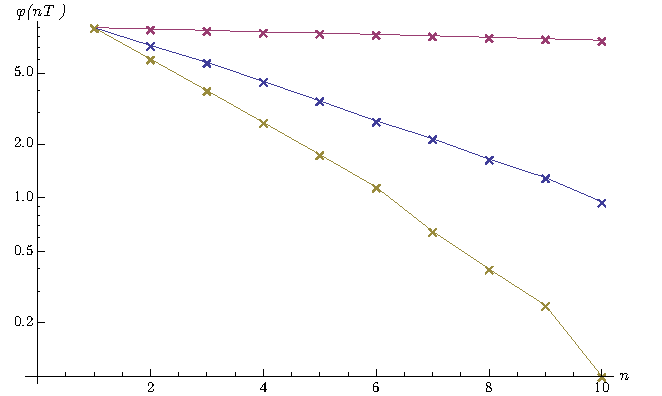
\includegraphics[width=13cm]{plot1.pdf}
\end{center}

\subsubsection*{Verh\"altnis aufeinanderfolgender Werte}
Nach der Annahme, dass $\varphi(t) \approx e^{-\alpha t}$ w\"urde man annehmen, dass das Verh\"altnis zweier aufeinanderfolgenden Werte konstant bleibt.
\vspace{10pt}

Ohne D\"ampfung
\begin{center}
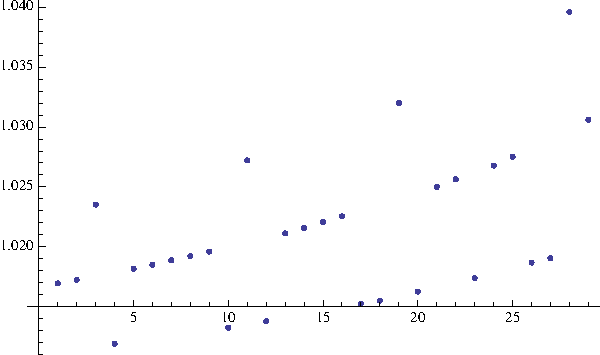
\includegraphics[width=13cm]{plot11.pdf}
\end{center}

\newpage
Mit D\"ampfung von 0.45A bzw. 0.6A
\begin{center}
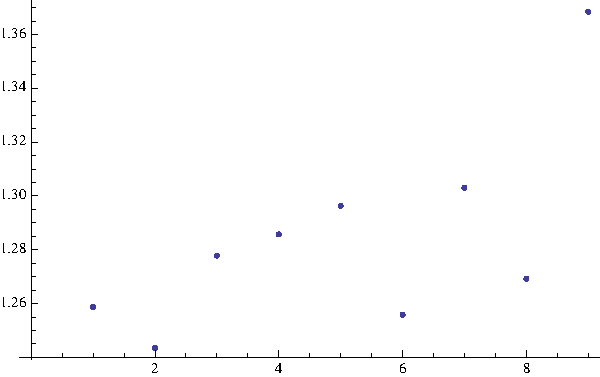
\includegraphics[width=6cm]{plot12.pdf}
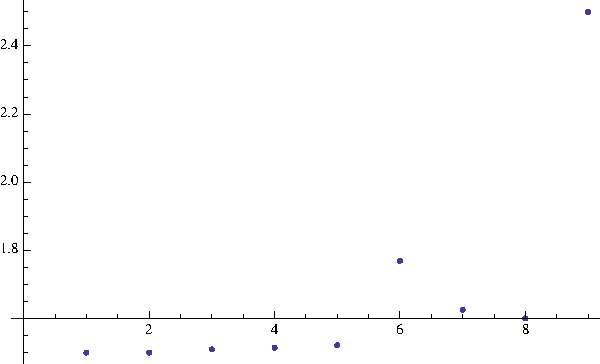
\includegraphics[width=6cm]{plot13.pdf}
\end{center}

%%
% Experiment 1I
%%
\section*{Experiment II}

% Aufbau und Ablauf
\subsection*{Aufbau und Ablauf}
Der Aufbau ist gleich wie bei Experiment I. Im Gegensatz zu Experiment I hat der Motor ein zus\"atzliches externes Moment geliefert. 
Zuerst haben wir die Resonanzfrequenz $\Omega_R$ mit der Abgesch\"atztung von $\alpha$ bestimmt. Dadurch konnten wir die maximale Amplitude bestimmen und in dieser Umgebung mehrere Punkte messen.
Dabei hat Patricia zus\"atzlich die Geschwindigkeit des Motors geregelt.

% Rohdaten
\subsection*{Rohdaten}
\subsubsection*{Ohne D\"ampfung}
\begin{tabular}{|l|l|l|l|l|l|l|l|l|l|l|}
\hline
$10T$[s]&19.1&20.0&20.5&22.0&21.0&18.5&19.5\\
\hline
$A$&4.1&8.6&4.3&1.7&2.9&1.5&6.0\\
\hline
\end{tabular}

\subsubsection*{Mit D\"ampfung 0.45A}
\begin{tabular}{|l|l|l|l|l|l|l|l|l|l|l|}
\hline
$10T$[s]&20.5&19.0&19.5&20.0&20.2&18.2&19.1\\
\hline
$A$&3.5&1.5&2.9&3.5&3.6&1.2&2.5\\
\hline
\end{tabular}

\subsubsection*{Mit D\"ampfung 0.6A}
\begin{tabular}{|l|l|l|l|l|l|l|l|l|l|l|}
\hline
$10T$[s]&22.0&20.0&18.0&16.0&21.0&21.5&19.0&20.5\\
\hline
$A$&1.3&2.1&1.1&0.5&1.9&1.7&1.4&2.1\\
\hline
\end{tabular}

% Auswertung
\subsection*{Auswertung}
Die Werte der einzelnen Messungen werden jeweils mit einer Ann\"aherung der Formel \ref{eq:a} dargestellt.
\subsubsection*{Ohne D\"ampfung}
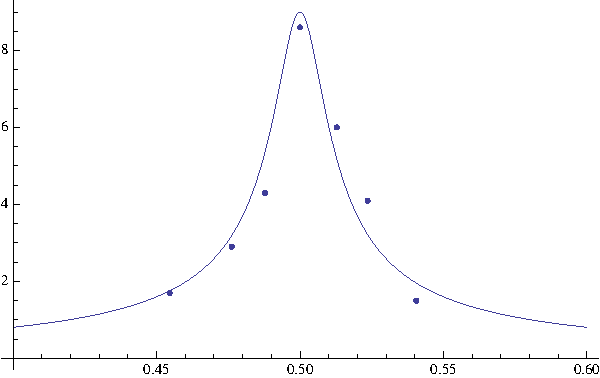
\includegraphics[width=13cm]{plot23.pdf}
\subsubsection*{Mit D\"ampfung 0.45A}
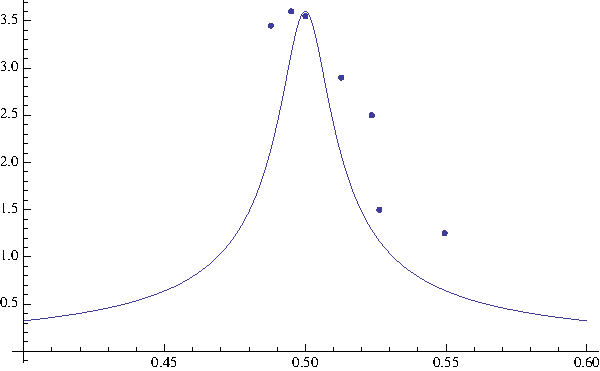
\includegraphics[width=13cm]{plot22.pdf}
\subsubsection*{Mit D\"ampfung 0.6A}
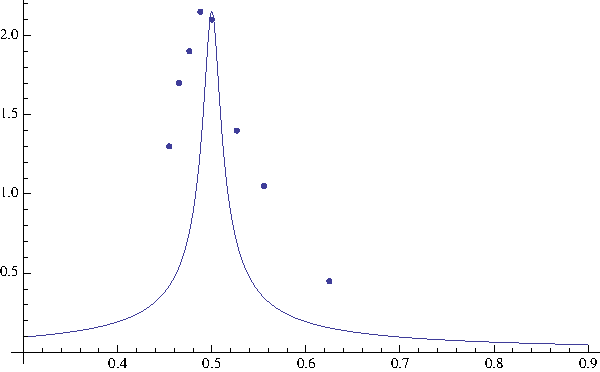
\includegraphics[width=13cm]{plot21.pdf}

%%
% Experiment 3
%%
\section*{Aufgabe III}
Die D\"ampfungskonstante $\alpha$ soll auf zwei verschiedene Arten bestimmt werden.\\
1. $\varphi(t) \approx e^{-\alpha t}$ \\
2. $\frac{A_{max}}{\sqrt{2}}$\\

% Auswertung
\subsection*{Teilaufgabe I}
Als Steigung der Gerade wird jeweils der erste und letzte Messwert verwendet.
\subsubsection*{Ohne D\"ampfung}
\[ \alpha = 1.7013 \]
\subsubsection*{Mit D\"ampfung 0.45A}
\[ \alpha = 0.4551 \]
\subsubsection*{Mit D\"ampfung 0.6A}
\[ \alpha = 0.2222 \]

% Zusammenfassung
\subsection*{Teilaufgabe II}
Die Werte werden direkt von den Darstellugen aus Aufgabe II abgelesen.
\subsubsection*{Ohne D\"ampfung}
\[ \alpha = 1.7013 \]
\subsubsection*{Mit D\"ampfung 0.45A}
\[ \alpha = 0.03 \]
\subsubsection*{Mit D\"ampfung 0.6A}
\[ \alpha = 0.04 \]

%%
% Diskussion
%%
\section*{Diskussion}
Bei Experiment I bildeten die Amplituden wie erwartet im logarithmischen Plot eine Gerade, nur mit sehr starker D\"ampfung wichen die Werte immer weiter von der Geraden ab. Dies liegt daran, dass das Pendel bereits nach zehn Schwingungen fast komplett stillsteht ($A <$ 0.1). Das Verh\"altnis der aufeinanderfolgenden Werte war nicht wie erwartet konstant, sondern scheint exponentiell zu steigen und aufgrund der groben Skala zwischen drei Kurven hin und her zu springen. Die wird wahrscheinlich durch einige vernachl\"assigte Faktoren der Apparatur verursacht. Die Werte des zweiten Experiments beschreiben alle einigermassen eine Kurve wie man sie erwarten w\"urde, die von uns gezeichnete Kurve die wir der maximalen Amplitude und der gesch\"atzten D\"ampfungskonstante angepasst haben treffen sie allerdings nicht immer sehr genau. Die Sch\"atzung der Resonanzfrequenz stimmte in allen F\"allen relativ gut mit der Realtit\"at \"uberein. Bei der dritten Aufgabe konnte die D\"ampfungskonstante aus der Steigung der Darstellung aus Experiment I relativ gut berechnet werden, das ablesen direkt aus den Darstellungen in Experiment II ergab sehr ungenaue Werte die wir uns soweit nicht erkl\"aren k\"onnen.

\end{document}